% ------------------------------------------------------------------------------
% TYPO3 CMS 7.0 - What's New - Chapter "Backend User Interface" (English Version)
%
% @author	Michael Schams <schams.net>
% @license	Creative Commons BY-NC-SA 3.0
% @link		http://typo3.org/download/release-notes/whats-new/
% @language	English
% ------------------------------------------------------------------------------
% LTXE-CHAPTER-UID:		41a3b97a-91f92c1d-c2e8aade-24735983
% LTXE-CHAPTER-NAME:	Backend User Interface
% ------------------------------------------------------------------------------

\section{Gebruikersinterface backend}

% ------------------------------------------------------------------------------
% LTXE-SLIDE-START
% LTXE-SLIDE-UID:		2bbdaa20-4676fe3f-ae8187b6-01b4c64d
% LTXE-SLIDE-ORIGIN:	fcbdd27c-e9005dff-0f4dd846-000ea412 English
% LTXE-SLIDE-TITLE:		In General
% LTXE-SLIDE-REFERENCE:	https://forge.typo3.org/issues/62333
% LTXE-SLIDE-REFERENCE:	https://forge.typo3.org/issues/62995
% LTXE-SLIDE-REFERENCE:	https://forge.typo3.org/issues/62158
% LTXE-SLIDE-REFERENCE:	https://forge.typo3.org/issues/61454
% ------------------------------------------------------------------------------

\begin{frame}[fragile]
	\frametitle{Gebruikersinterface backend}
	\framesubtitle{Algemeen}

	\begin{itemize}
		\item De gebruikersinterface van de backend heeft een ander uiterlijk
		\item Gebaseerd op Twitter Bootstrap versie 3.2.x
		\item Alle iconen zijn nieuw gemaakt en uitgevoerd in "tegel"-stijl
		\item Iconen gebruiken Font Awesome versie 4.2.x
		\item Functiemenu aan de linkerzijde is aangepast
		\item Iconen in het functiemenu gebruiken een plat ontwerp, kleurige achtergrond,
			monochroom/negatief pictogram in de voorgrond, afgeronde hoeken
		\item Breedte van functiemenu kan verkleind worden zodat alleen iconen zichtbaar zijn

	\end{itemize}

\end{frame}

% ------------------------------------------------------------------------------
% LTXE-SLIDE-START
% LTXE-SLIDE-UID:		6aebd5d2-769d14fa-28f03cc5-6e0bc8be
% LTXE-SLIDE-ORIGIN:	0ae980b6-0d2ae6c6-52182f58-aaef69e3 English
% LTXE-SLIDE-TITLE:		Look & Feel (1)
% ------------------------------------------------------------------------------

\begin{frame}[fragile]
	\frametitle{Gebruikersinterface backend}
	\framesubtitle{Uiterlijk}

	\begin{figure}
		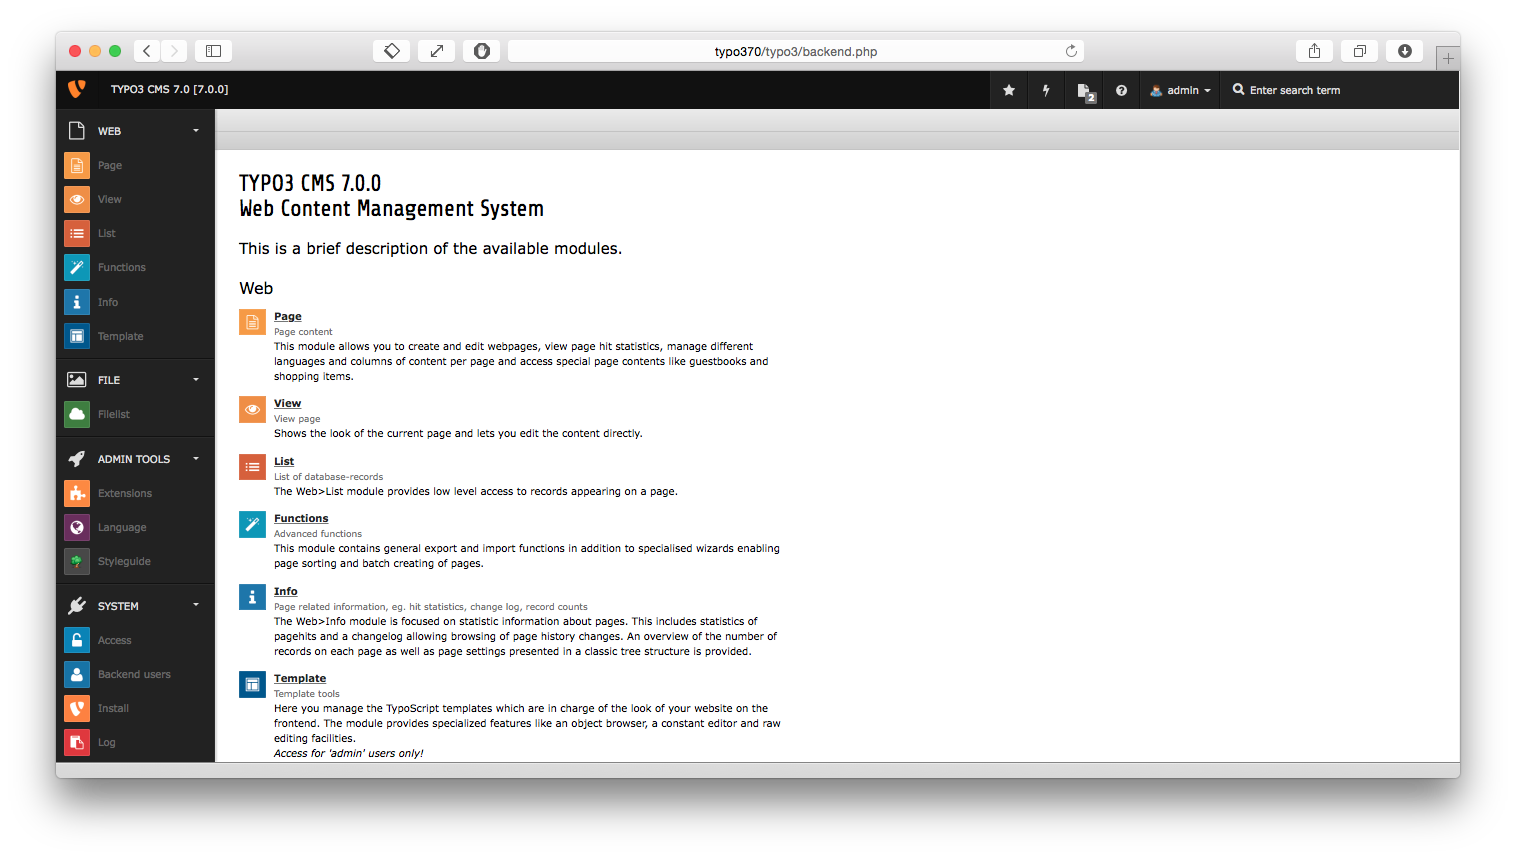
\includegraphics[width=0.90\linewidth]{BackendUserInterface/be-totalscreenshot1.png}
	\end{figure}

\end{frame}

% ------------------------------------------------------------------------------
% LTXE-SLIDE-START
% LTXE-SLIDE-UID:		8ff1b087-7a3d4d5d-d121e1c5-4cc34fef
% LTXE-SLIDE-ORIGIN:	250b123b-2c0bfce4-506f16b0-629baa10 English
% LTXE-SLIDE-TITLE:		Look & Feel (2)
% ------------------------------------------------------------------------------

\begin{frame}[fragile]
	\frametitle{Gebruikersinterface backend}
	\framesubtitle{Uiterlijk}

	\begin{figure}
		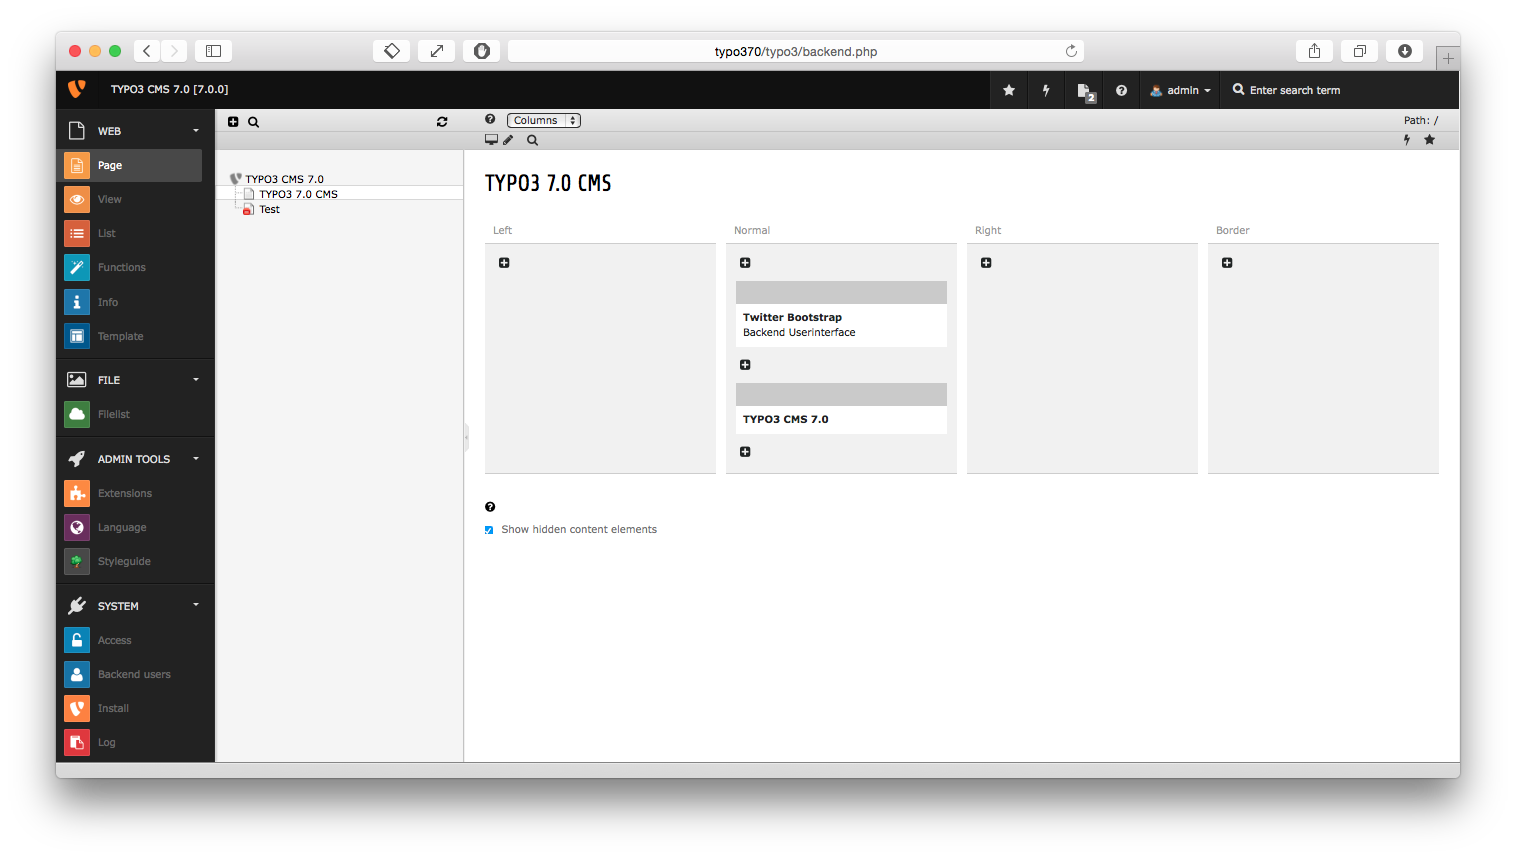
\includegraphics[width=0.90\linewidth]{BackendUserInterface/be-totalscreenshot2.png}
	\end{figure}

\end{frame}

% ------------------------------------------------------------------------------
% LTXE-SLIDE-START
% LTXE-SLIDE-UID:		31d7f9d8-f5b70f11-f28ce33e-813d9518
% LTXE-SLIDE-ORIGIN:	2d4d33ee-071ae6ed-9f4d0c04-49361364 English
% LTXE-SLIDE-TITLE:		Look & Feel (3)
% ------------------------------------------------------------------------------

\begin{frame}[fragile]
	\frametitle{Gebruikersinterface backend}
	\framesubtitle{Uiterlijk}

	\begin{figure}
		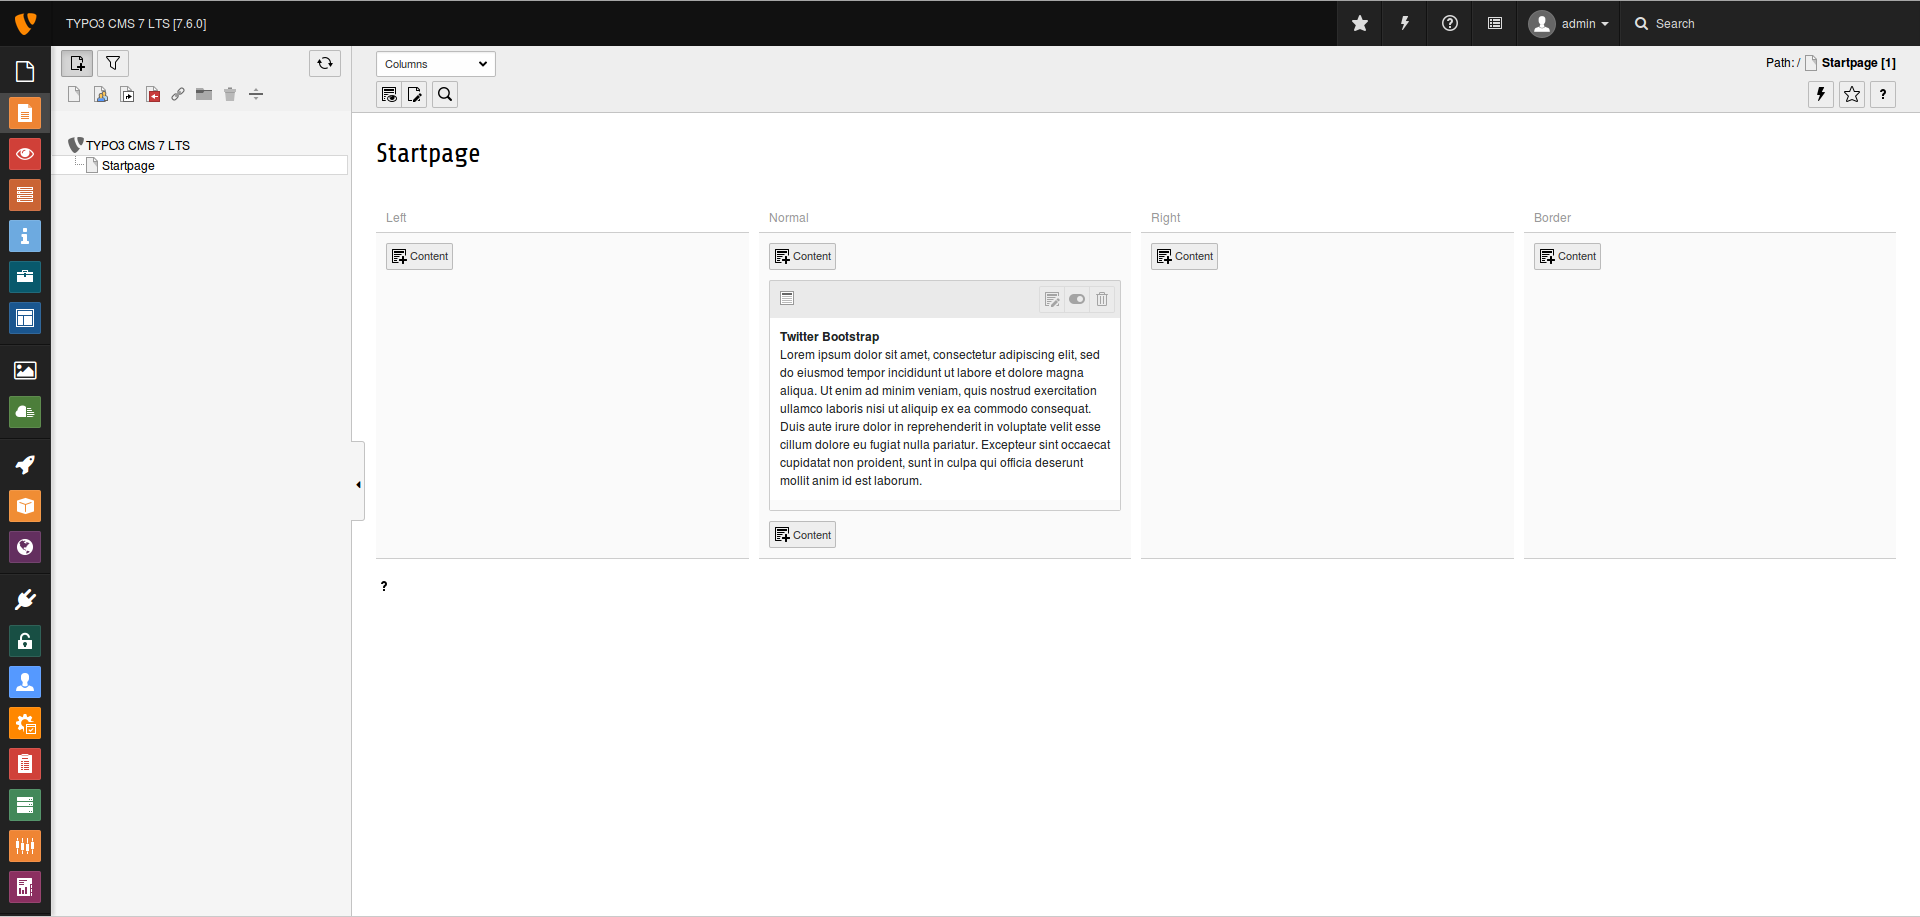
\includegraphics[width=0.90\linewidth]{BackendUserInterface/be-totalscreenshot3.png}
	\end{figure}

\end{frame}

% ------------------------------------------------------------------------------
% LTXE-SLIDE-START
% LTXE-SLIDE-UID:		6bb8152c-f7e62596-389be15e-be2337ef
% LTXE-SLIDE-ORIGIN:	de58d070-98483f3d-0949f2d1-856a9e7e English
% LTXE-SLIDE-TITLE:		Backend User Login
% ------------------------------------------------------------------------------

\begin{frame}[fragile]
	\frametitle{Gebruikersinterface backend}
	\framesubtitle{Aanmeldscherm backend}

	\begin{figure}
		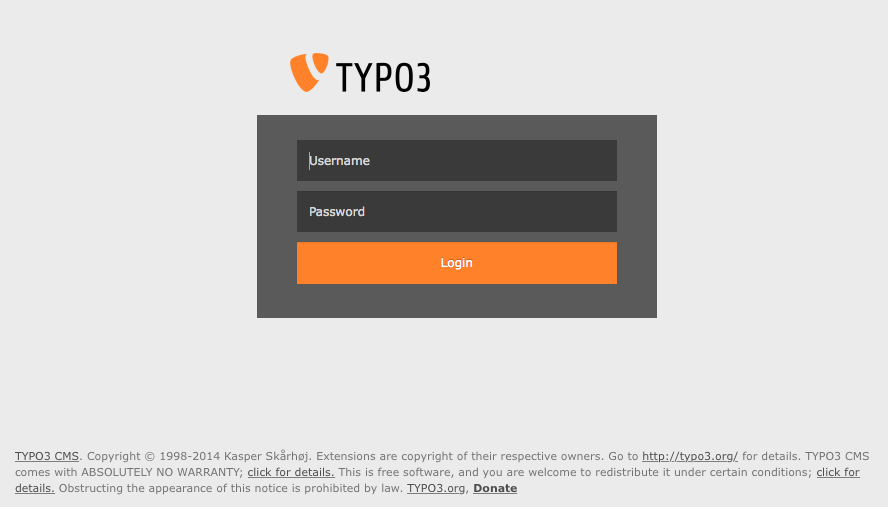
\includegraphics[width=0.80\linewidth]{BackendUserInterface/be-login.png}
	\end{figure}

\end{frame}

% ------------------------------------------------------------------------------
% LTXE-SLIDE-START
% LTXE-SLIDE-UID:		63363226-ab981023-6ecdf9f9-c48033b4
% LTXE-SLIDE-ORIGIN:	9baa13c8-78b2f416-28da8e3d-b234e7dc English
% LTXE-SLIDE-TITLE:		Refactor & recolor Modul Menu (Bootstrap)
% LTXE-SLIDE-REFERENCE:	https://forge.typo3.org/issues/62353
% ------------------------------------------------------------------------------

\begin{frame}[fragile]
	\frametitle{Gebruikersinterface backend}
	\framesubtitle{Bovenbalk (Modulemenu)}

	\begin{figure}
		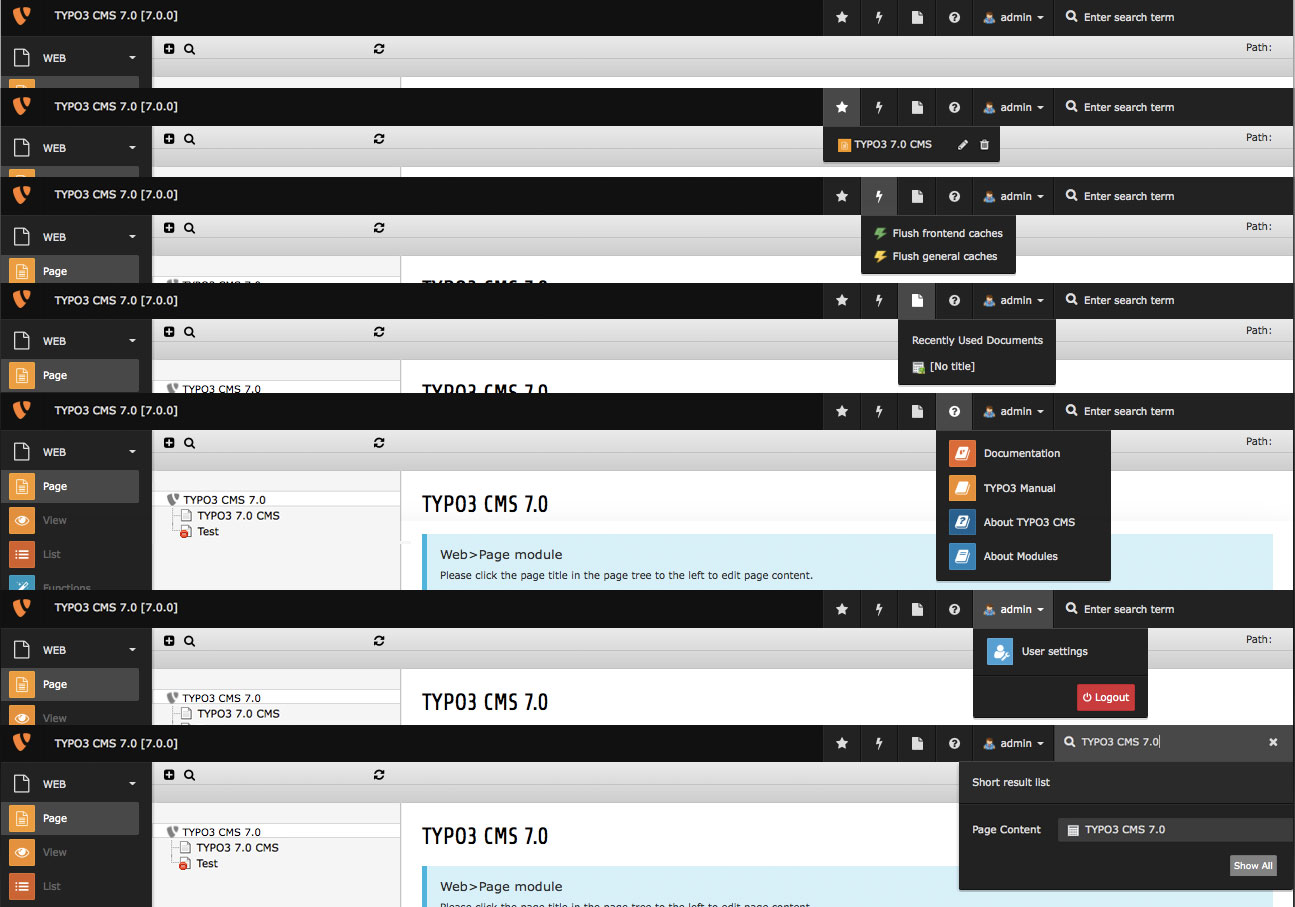
\includegraphics[width=0.70\linewidth]{BackendUserInterface/be-topbar.jpg}
	\end{figure}

\end{frame}

% ------------------------------------------------------------------------------
% LTXE-SLIDE-START
% LTXE-SLIDE-UID:		93eb9356-e3b84d90-c6797b0e-ed88a0da
% LTXE-SLIDE-ORIGIN:	4369ae5e-948d1afa-8212cd72-c91c660b English
% LTXE-SLIDE-TITLE:		New List Module Styling
% LTXE-SLIDE-REFERENCE:	https://forge.typo3.org/issues/62963
% ------------------------------------------------------------------------------

\begin{frame}[fragile]
	\frametitle{Gebruikersinterface backend}
	\framesubtitle{Lijstmodule en klembord}

	\begin{figure}
		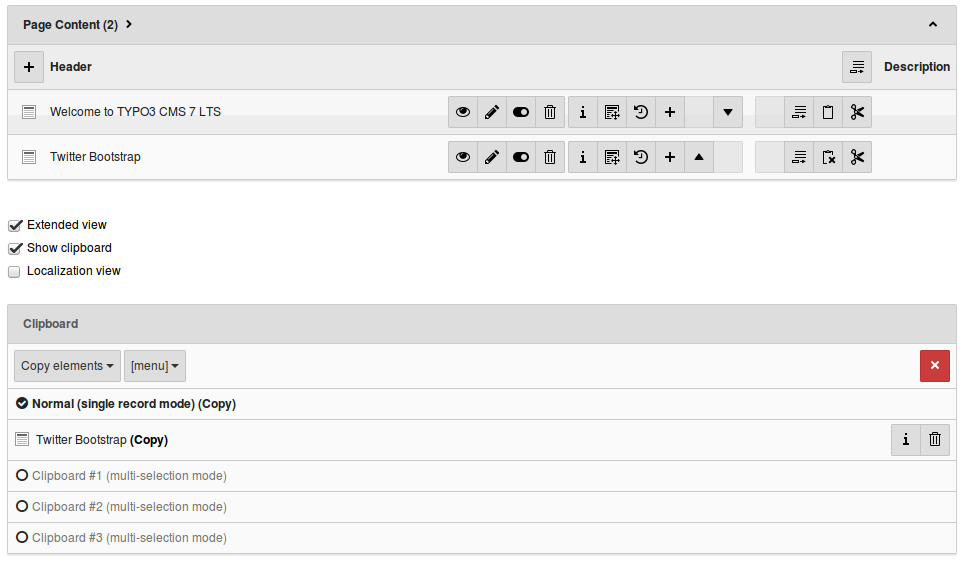
\includegraphics[width=0.80\linewidth]{BackendUserInterface/be-list.png}
	\end{figure}

\end{frame}

% ------------------------------------------------------------------------------
% LTXE-SLIDE-START
% LTXE-SLIDE-UID:		90bf5106-96589244-178897f2-fcbb2487
% LTXE-SLIDE-ORIGIN:	252361f7-e5c42ec2-a90ecd64-4331f02b English
% LTXE-SLIDE-TITLE:		Table Style
% LTXE-SLIDE-REFERENCE:	https://forge.typo3.org/issues/62159
% ------------------------------------------------------------------------------

\begin{frame}[fragile]
	\frametitle{Gebruikersinterface backend}
	\framesubtitle{Tabelstijl}

	\begin{figure}
		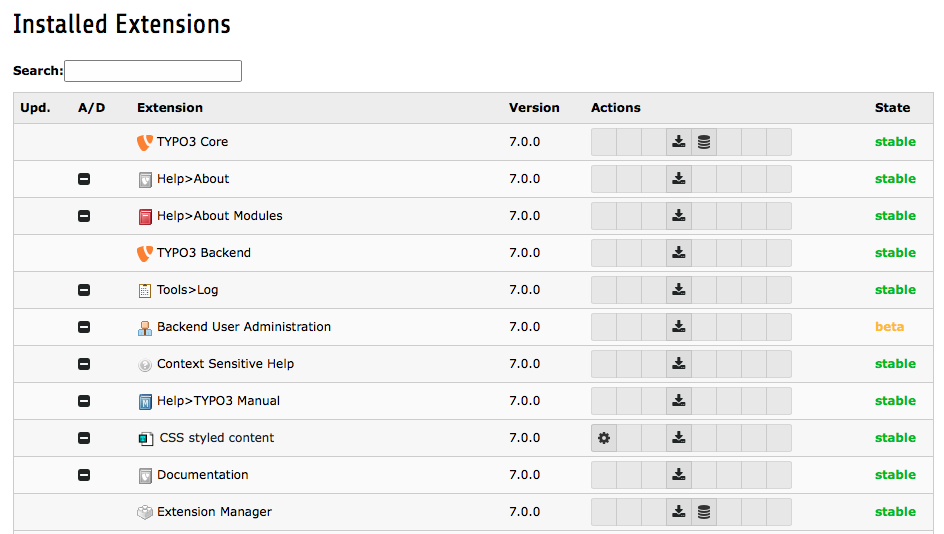
\includegraphics[width=0.99\linewidth]{BackendUserInterface/be-table.png}
	\end{figure}

\end{frame}

% ------------------------------------------------------------------------------
% LTXE-SLIDE-START
% LTXE-SLIDE-UID:		e75e9e8a-75c010ef-98c70794-47c6ade1
% LTXE-SLIDE-ORIGIN:	785f717d-a7c4d1dd-f186ca6a-060c1dc4 English
% LTXE-SLIDE-TITLE:		Page And List Search
% LTXE-SLIDE-REFERENCE:	https://forge.typo3.org/issues/59763
% ------------------------------------------------------------------------------

\begin{frame}[fragile]
	\frametitle{Gebruikersinterface backend}
	\framesubtitle{Zoeken in lijst- en paginamodule}

	\begin{itemize}
		\item Met een klik op het vergrootglas is een zoekbalk beschikbaar in de lijst- en paginamodule\newline
			(zoekfunctie zat vroeger onderaan de pagina)
	\end{itemize}

	\begin{figure}
		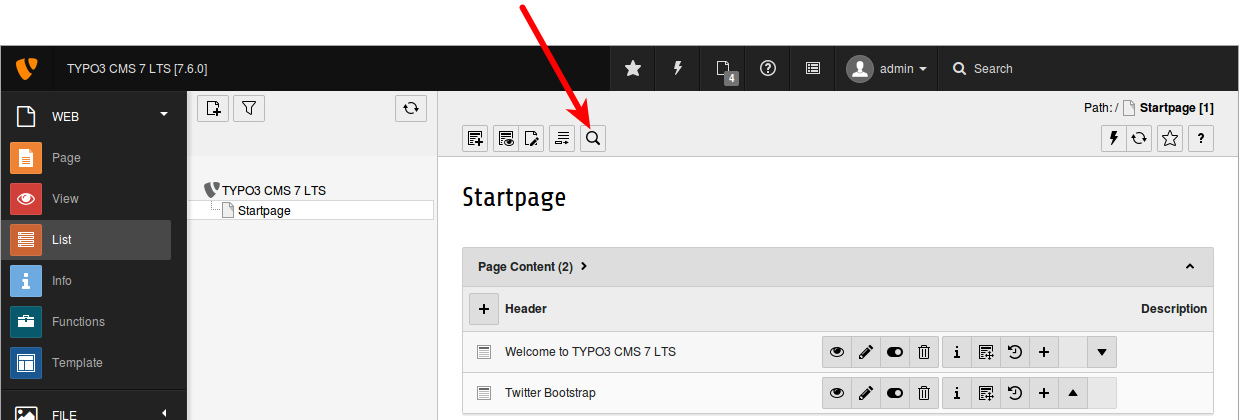
\includegraphics[width=0.95\linewidth]{BackendUserInterface/be-search.jpg}
	\end{figure}

\end{frame}

% ------------------------------------------------------------------------------
% LTXE-SLIDE-START
% LTXE-SLIDE-UID:		7827e3db-b8ff02e6-9af079b5-b0eeff1f
% LTXE-SLIDE-ORIGIN:	df97fbbf-9ea6c6a9-d9b4c5d4-f8fe1601 English
% LTXE-SLIDE-TITLE:		Migrate Counter of Open Documents to Bootstrap "Badge"
% LTXE-SLIDE-REFERENCE:	https://forge.typo3.org/issues/61675
% ------------------------------------------------------------------------------

\begin{frame}[fragile]
	\frametitle{Gebruikersinterface backend}
	\framesubtitle{Schildje toont open documenten}

	\begin{itemize}
		\item Het aantal open documenten is te zien op een Bootstrap "schild"\newline
			(vereist systeemextensie "Open documenten")
	\end{itemize}
	\begin{figure}
		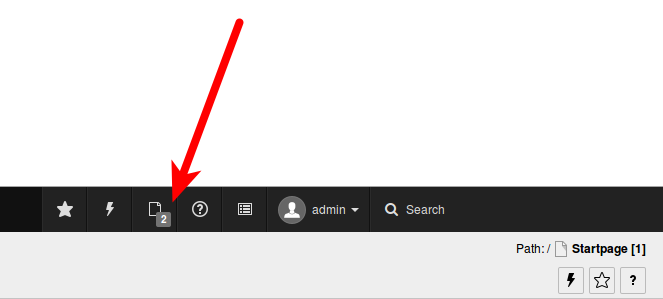
\includegraphics[width=0.75\linewidth]{BackendUserInterface/be-badge.png}
	\end{figure}

\end{frame}

% ------------------------------------------------------------------------------
% LTXE-SLIDE-START
% LTXE-SLIDE-UID:		bee90e9f-0731c23d-a62cc396-e1e4137c
% LTXE-SLIDE-ORIGIN:	a25faae4-8c12c45e-b337b64a-0cf2f53f English
% LTXE-SLIDE-TITLE:		Rebrush FlashMessage
% LTXE-SLIDE-REFERENCE:	https://forge.typo3.org/issues/62580
% ------------------------------------------------------------------------------

\begin{frame}[fragile]
	\frametitle{Gebruikersinterface backend}
	\framesubtitle{Statusberichten}

	\begin{itemize}
		\item Het uiterlijk van statusberichten is bijgewerkt
		\item Contrast tussen tekst en achtergrond is verbeterd
	\end{itemize}

	\begin{columns}[T]
		\begin{column}{.25\textwidth}
			\smaller\hfill 
				\begingroup\color{typo3red}TYPO3 CMS < 7.0\endgroup
			\normalsize
		\end{column}

		\begin{column}{.5\textwidth}
			\begin{figure}\vspace*{-0.6cm}
				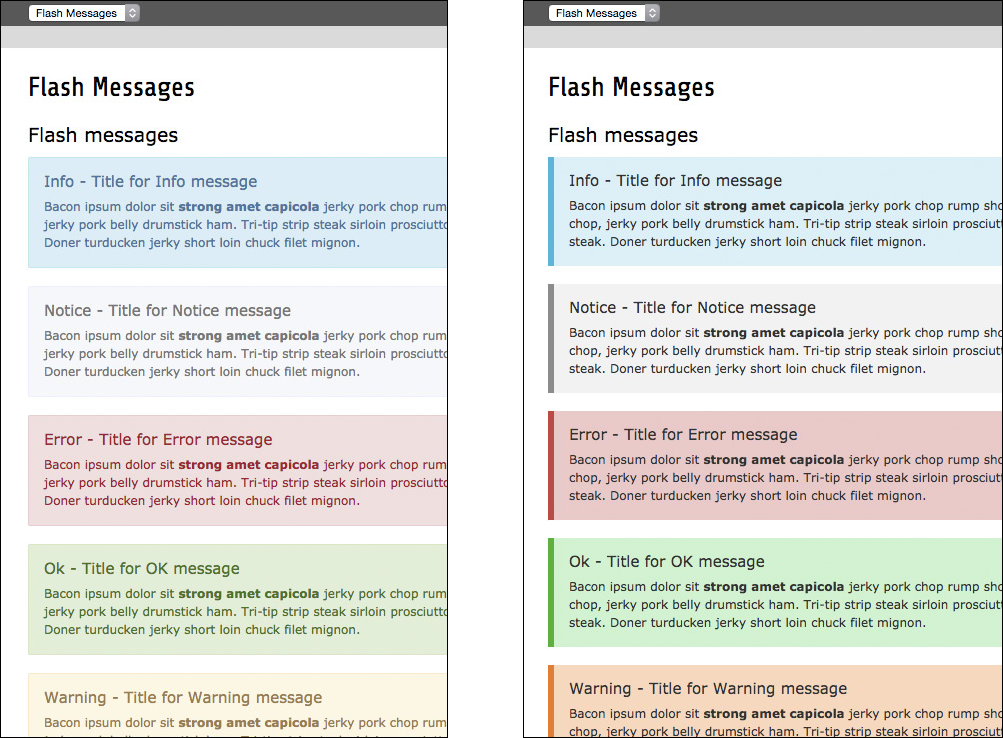
\includegraphics[width=0.99\linewidth]{BackendUserInterface/be-flashmessages.png}
			\end{figure}
		\end{column}

		\begin{column}{.25\textwidth}
			\smaller
				\begingroup\color{typo3red}TYPO3 CMS >= 7.0\endgroup
			\normalsize
		\end{column}

	\end{columns}

\end{frame}

% ------------------------------------------------------------------------------
% LTXE-SLIDE-START
% LTXE-SLIDE-UID:		4df8e8e8-55042f30-f766e06a-9e906c62
% LTXE-SLIDE-ORIGIN:	d6a85376-8109aa8c-45a40582-7edb975a English
% LTXE-SLIDE-TITLE:		Video Player in Info Window
% LTXE-SLIDE-REFERENCE:	https://forge.typo3.org/issues/61668
% ------------------------------------------------------------------------------

\begin{frame}[fragile]
	\frametitle{Gebruikersinterface backend}
	\framesubtitle{Videospeler in Infoscherm}
	\begin{itemize}
		\item HTML5 audio- en videobestanden kunnen in het infoscherm afgespeeld worden
			(waar metadata wordt afgebeeld)
		\begin{figure}
			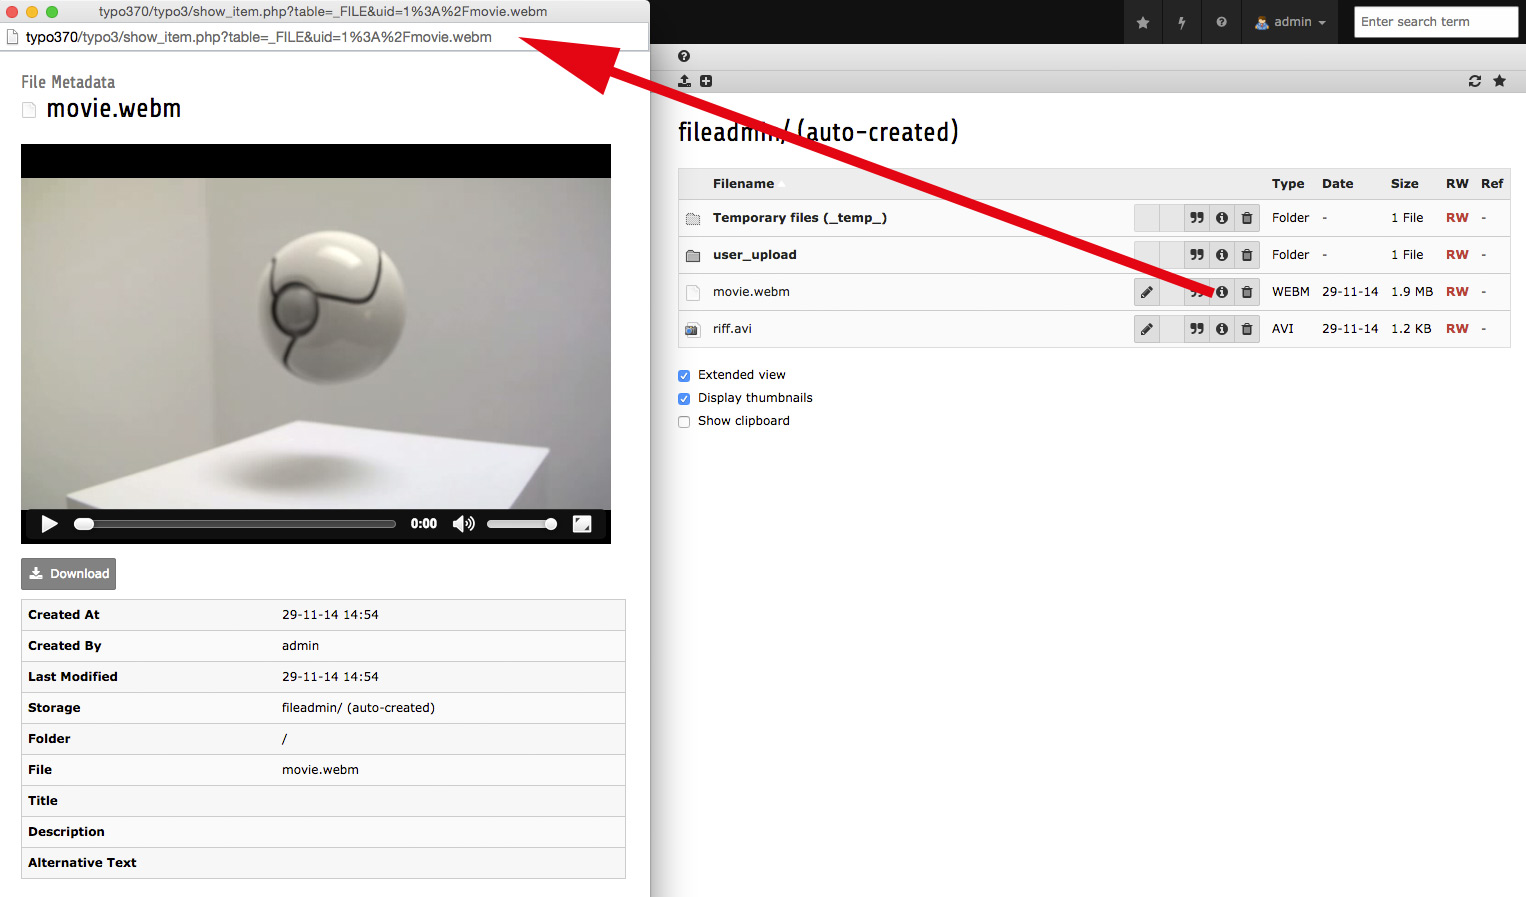
\includegraphics[width=0.70\linewidth]{BackendUserInterface/be-info.jpg}
		\end{figure}

	\end{itemize}

\end{frame}

% ------------------------------------------------------------------------------
